

The development of the web application focused on integrating the individual visualization components into a cohesive interactive system. The webapp's initial purpose was to test the realized visualizations in different scenarios quickly, allowing for rapid iteration and validation of design decisions, but it later became an integral part of the final project. The following sections describe the evolution of the user interface, coordination mechanisms between visualizations, and the various features implemented to support the explanation workflow, as well as the final product delivered to the users with its various mechanisms and ways of interaction with details about the integrations and inner mechanisms.

\section{Webapp evolutions}

The first development step toward an integrated system \cite{git7commit} involved creating the webapp preceding the coordinated visualizations. One of the first realized working versions, observable in Figure \ref{fig:firstWebapp}. This rudimentary version allowed users to select one of three datasets, choose a classifier, set its parameters, train the selected model using the chosen dataset, and display the data generated by $\text{LORE}_{sa}$. The two displayed plots were faithful to the generated data, but the coordination between them and the color mapping was not yet implemented.

\begin{figure}[htbp]
    \centering
    \begin{subfigure}[c]{0.49\textwidth}
        \centering
        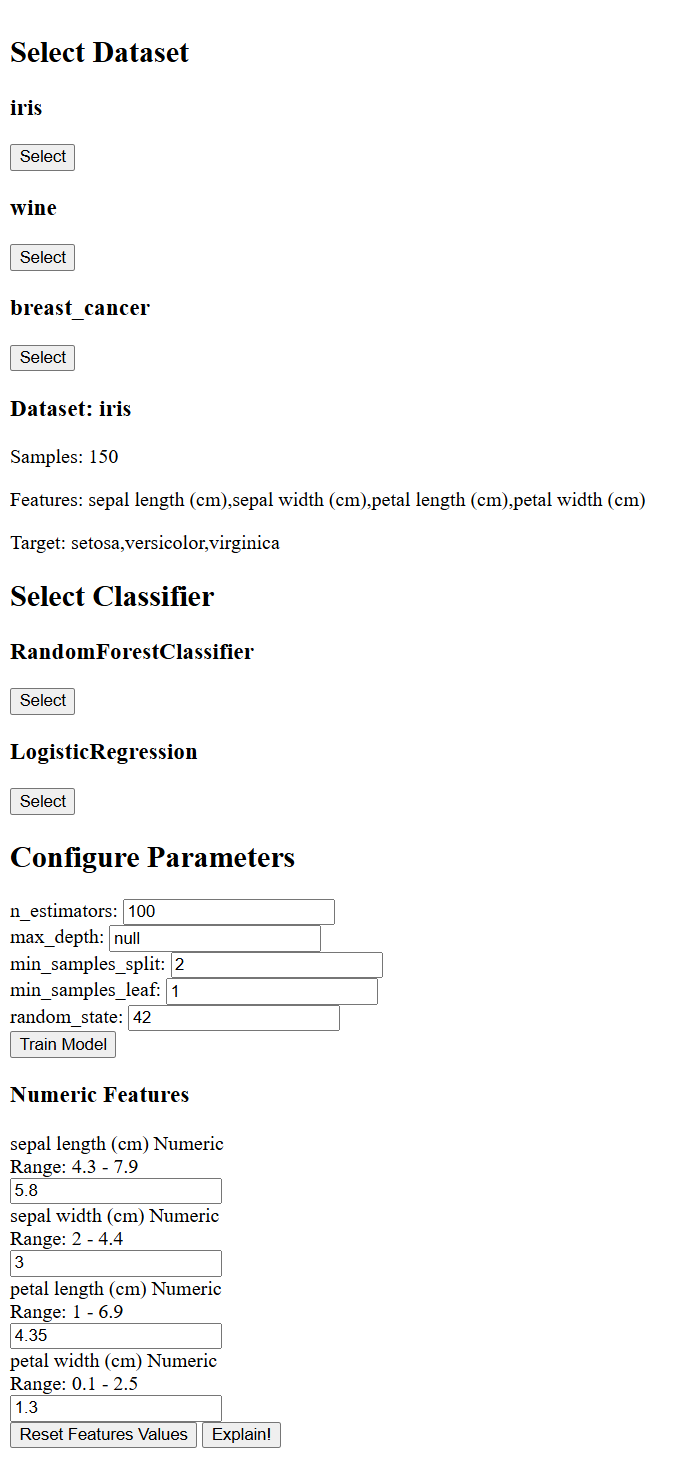
\includegraphics[width=\textwidth]{images/first webapp a.png}
        \caption{Selection process.}
    \end{subfigure}
    \hfill
    \begin{subfigure}[c]{0.49\textwidth}
        \centering
        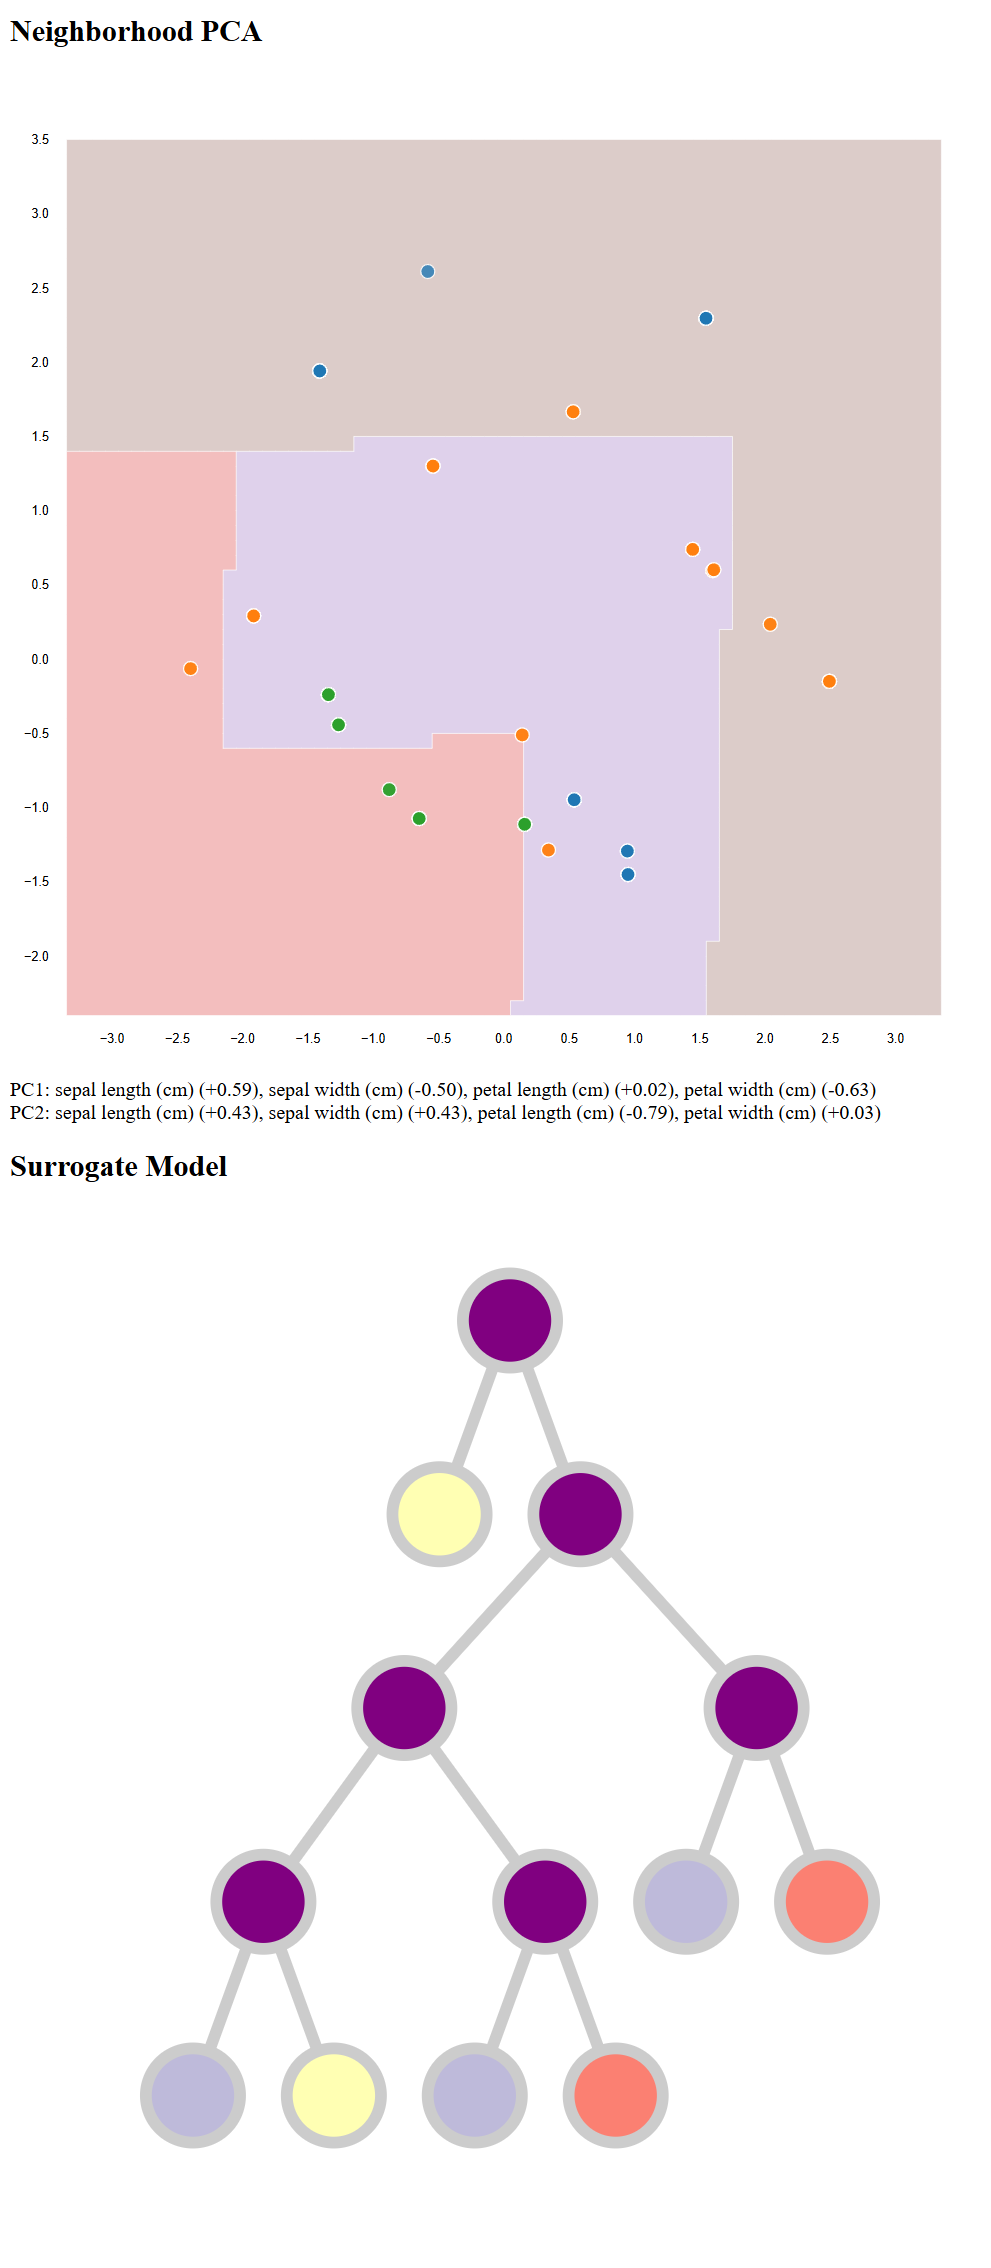
\includegraphics[width=\textwidth]{images/first webapp b.png}
        \caption{Generated plots.}
    \end{subfigure}
    \caption{Initial webapp prototype showing dataset selection interface and separate visualization components before coordination implementation.}
    \label{fig:firstWebapp}
\end{figure}

After this first implementation, several key features were developed: page styling \cite{git8commit}, hover interaction on the spatial neighborhood analysis plot \cite{git9commit}, click functionality on spatial neighborhood analysis plot points to highlight the rules path \cite{git10commit}, and bidirectional highlighting \cite{git11commit}. The first implementation of these described features can be observed in Figures \ref{fig:hover and highlight first scatter} and \ref{fig:hover and highlight first tree}.

\begin{figure}
    \centering
    \begin{subfigure}[c]{\textwidth}
        \centering
        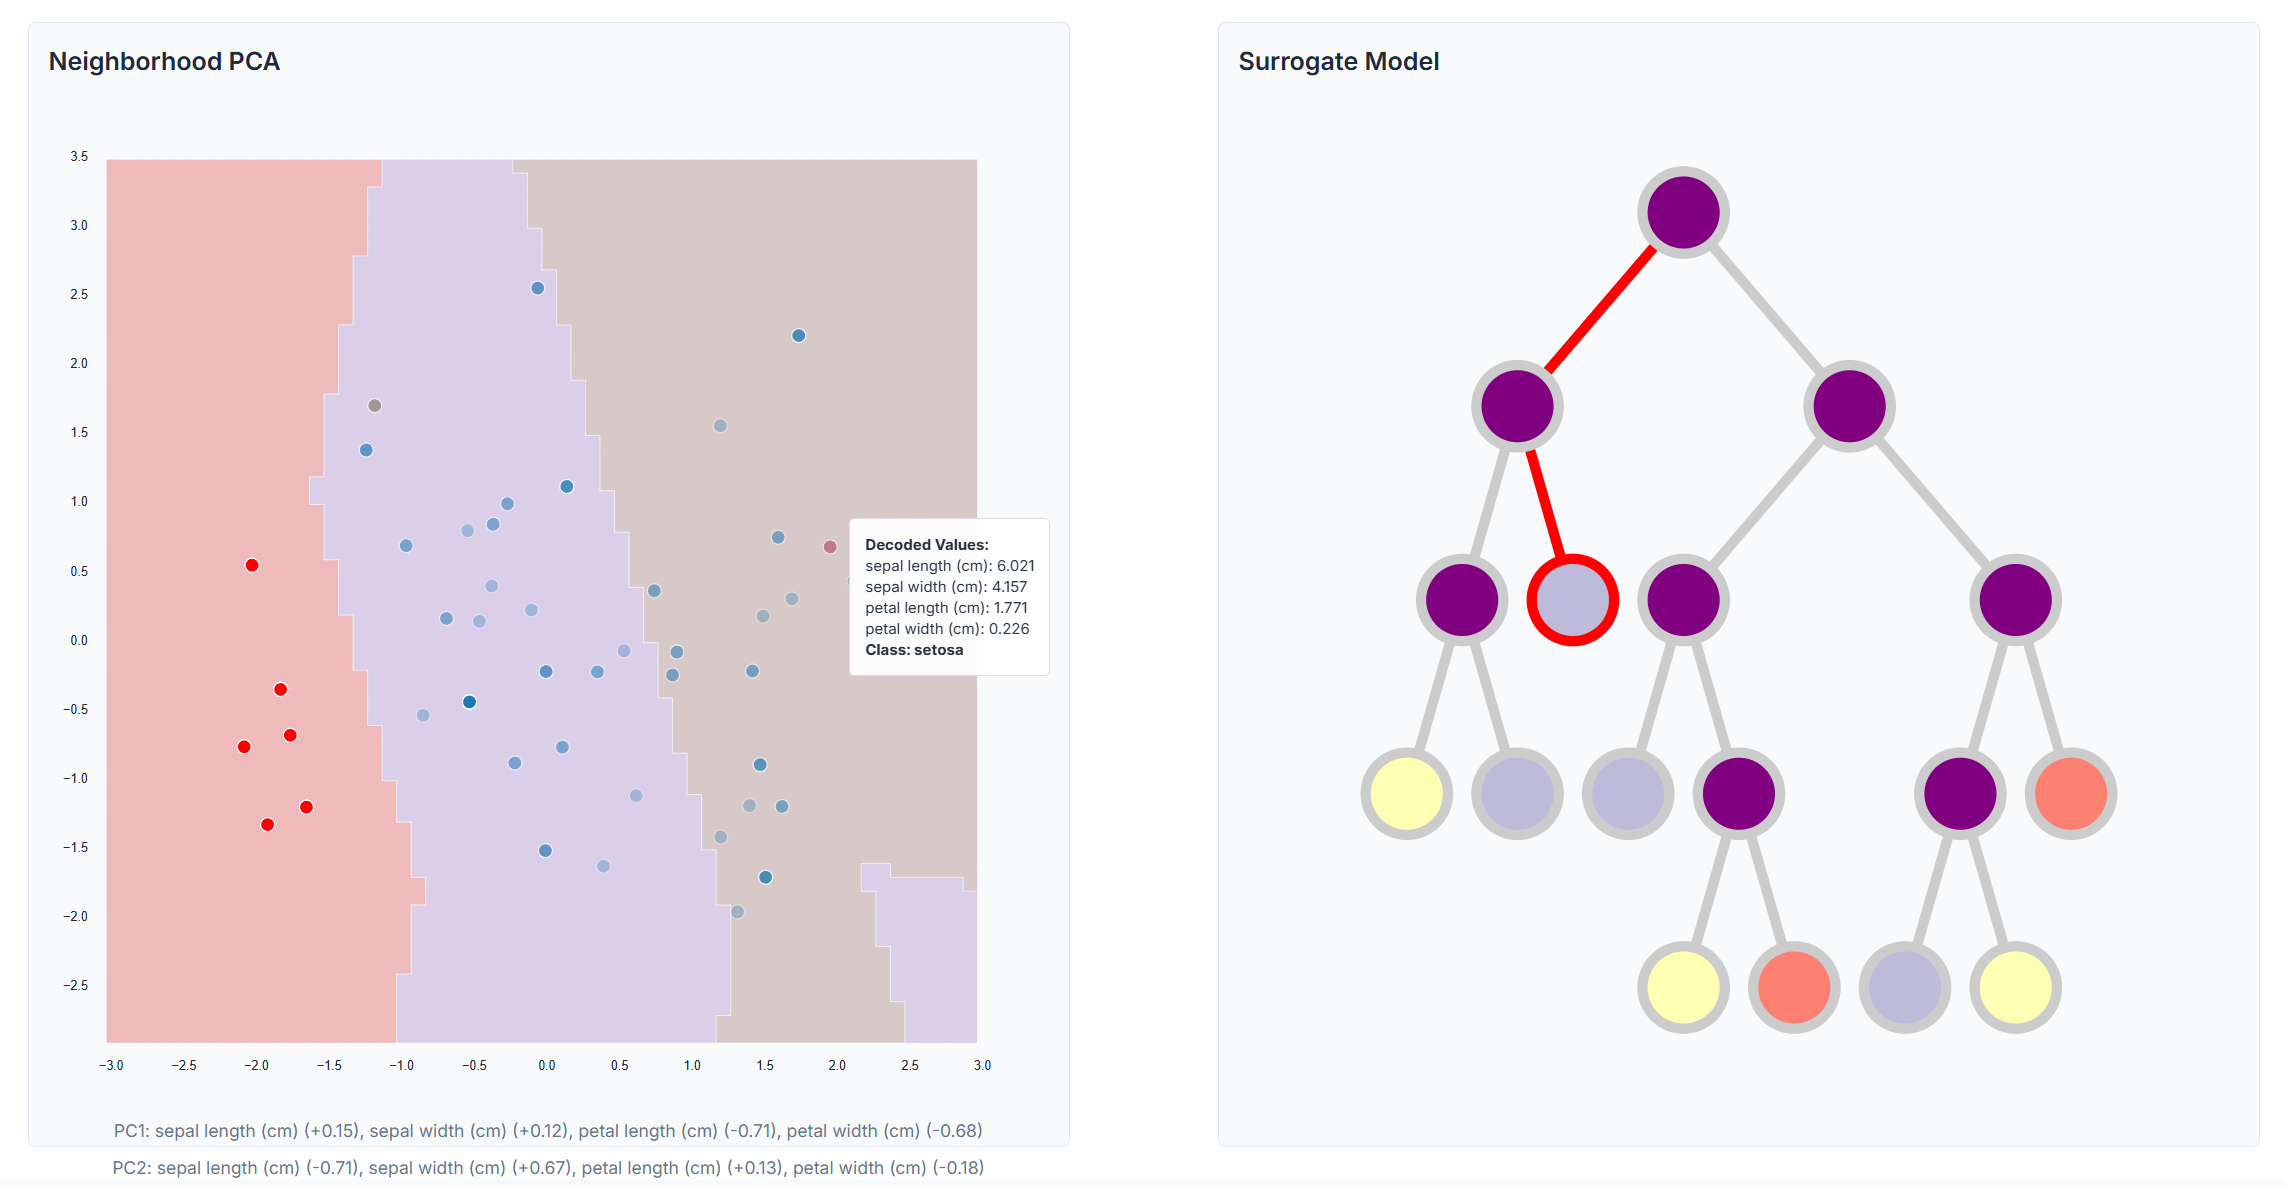
\includegraphics[width=\textwidth]{images/highlight points to leaf first.png}
        \caption{Hover and click on spatial neighborhood analysis plot.}
        \label{fig:hover and highlight first scatter}
    \end{subfigure}

    \begin{subfigure}[c]{\textwidth}
        \centering
        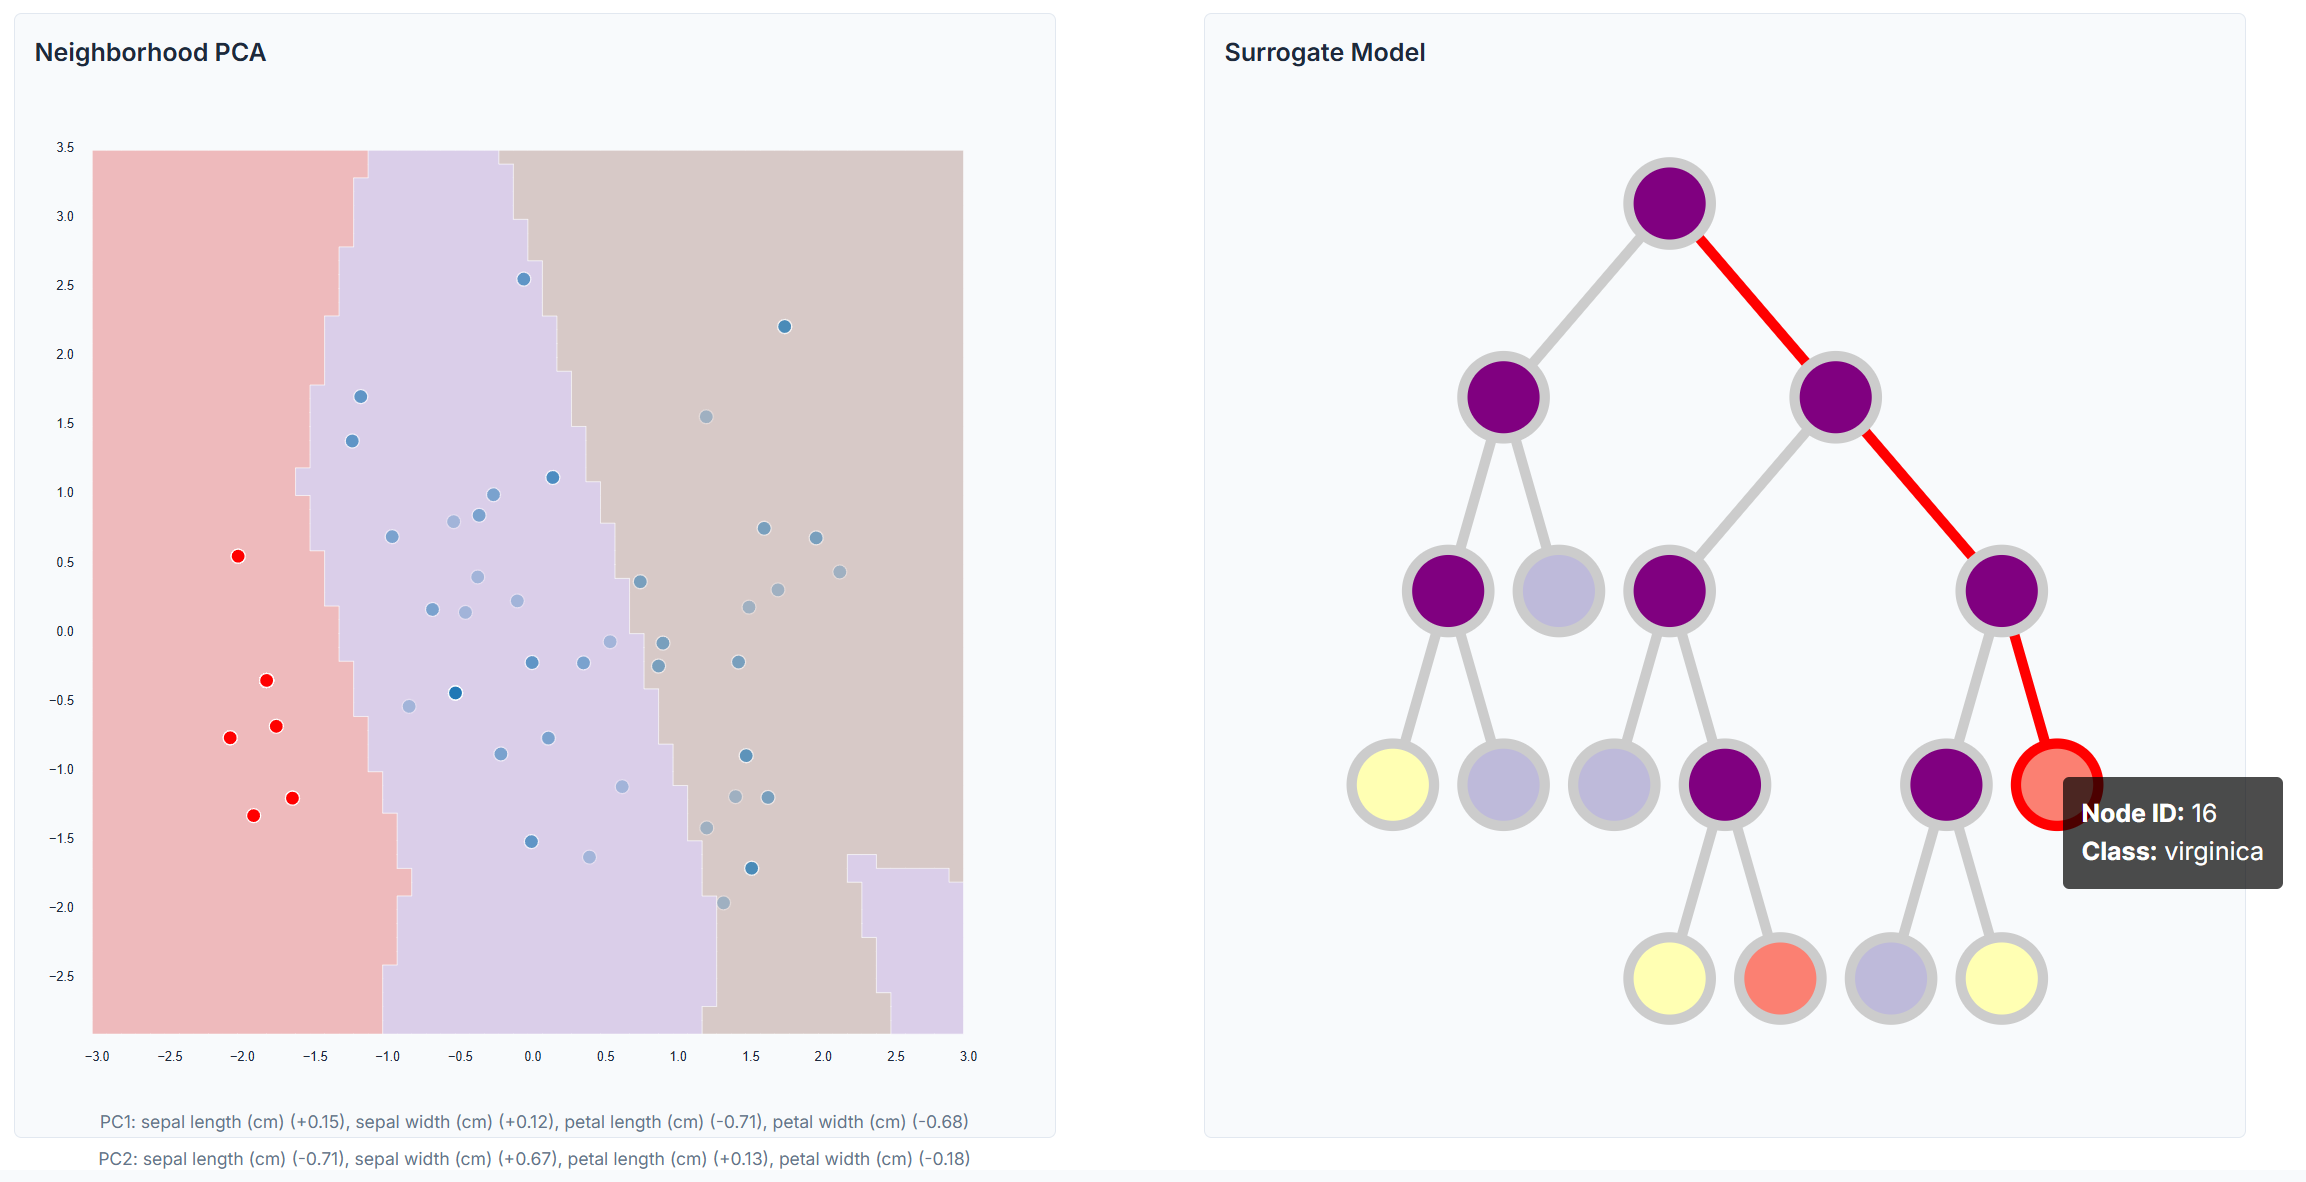
\includegraphics[width=\textwidth]{images/highlight leaf to points first.png}
        \caption{Hover and click on tree leaf.}
        \label{fig:hover and highlight first tree}
    \end{subfigure}

    \caption{Initial implementation of bidirectional coordination between spatial neighborhood analysis plot and surrogate model visualizations through interactive highlighting.}
    
\end{figure}

Subsequently, the webapp UI was improved \cite{git12commit, git16commit} and colors matched between the two visualizations \cite{git13commit} using the color palette shown in Table \ref{tab:firstColorPalette}, available on colorbrewer2.org \cite{colorbrewer2ColorPalette}. The explained instance was distinguished by giving it a different symbol (star) in the spatial neighborhood analysis plot to showcase its location relative to the generated neighborhood \cite{git14commit}. We also provided users with the ability to choose the neighborhood size and the granularity step for Voronoi tessellation \cite{git15commit}. The described state of the visualization is showcased in Figure \ref{fig:webappV2}.

\begin{table}[h]
    \centering
    \caption{First color palette used.}
    \label{tab:firstColorPalette}
    \renewcommand{\arraystretch}{2.5} % taller cells
    \setlength{\tabcolsep}{8pt}       % horizontal padding
    \begin{tabular}{
        |>{\centering\arraybackslash\columncolor[HTML]{8dd3c7}}m{3cm}
        |>{\centering\arraybackslash\columncolor[HTML]{ffffb3}}m{3cm}
        |>{\centering\arraybackslash\columncolor[HTML]{bebada}}m{3cm}
        |>{\centering\arraybackslash\columncolor[HTML]{fb8072}}m{3cm}|
    }
        \hline
        \#8dd3c7 & \#ffffb3 & \#bebada & \#fb8072 \\
        \hline
        \end{tabular}

    \begin{tabular}{
        |>{\centering\arraybackslash\columncolor[HTML]{80b1d3}}m{3cm}
        |>{\centering\arraybackslash\columncolor[HTML]{fdb462}}m{3cm}
        |>{\centering\arraybackslash\columncolor[HTML]{b3de69}}m{3cm}
        |>{\centering\arraybackslash\columncolor[HTML]{fccde5}}m{3cm}|
    }
        \hline
        \#80b1d3 & \#fdb462 & \#b3de69 & \#fccde5 \\
        \hline
    \end{tabular}

    \begin{tabular}{
        |>{\centering\arraybackslash\columncolor[HTML]{d9d9d9}}m{3cm}
        |>{\centering\arraybackslash\columncolor[HTML]{bc80bd}}m{3cm}
        |>{\centering\arraybackslash\columncolor[HTML]{ccebc5}}m{3cm}
        |>{\centering\arraybackslash\columncolor[HTML]{ffed6f}}m{3cm}|
    }
        \hline
        \#d9d9d9 & \#bc80bd & \#ccebc5 & \#ffed6f \\
        \hline
    \end{tabular}
\end{table}

\begin{figure}[htbp]
    \centering
    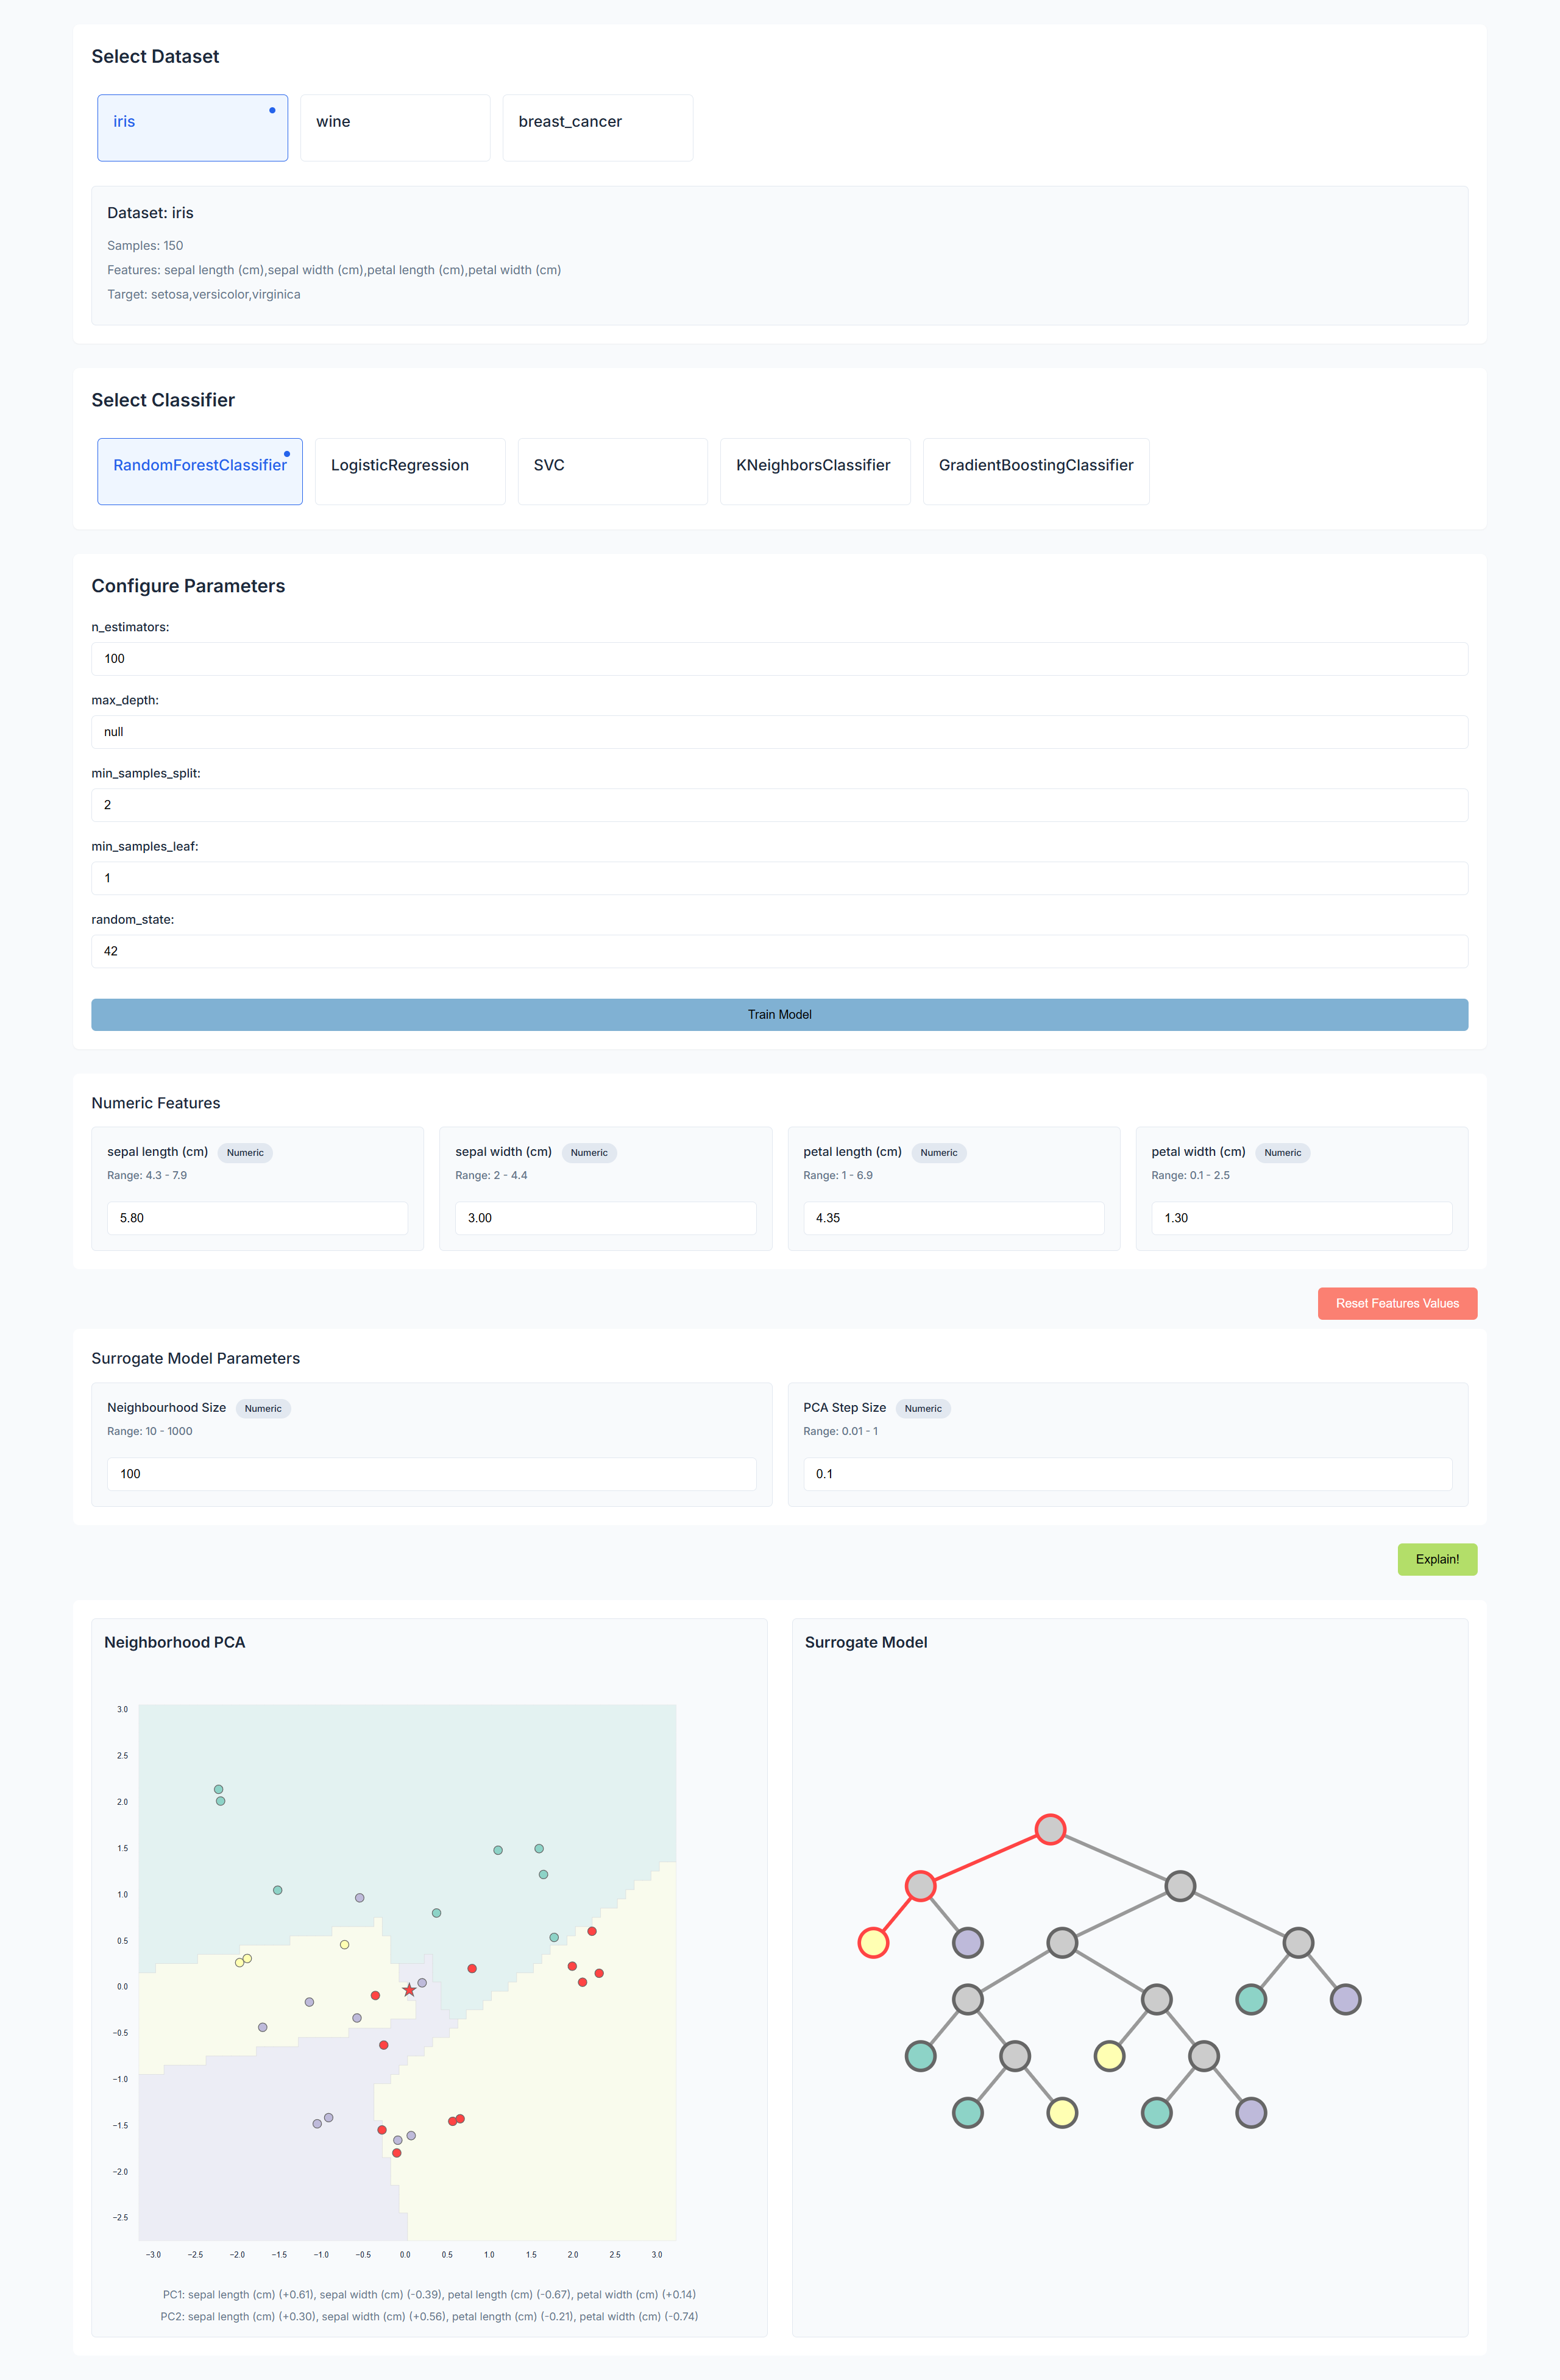
\includegraphics[width=0.8\textwidth]{images/webapp improved look overall.png}
    \caption{Refined webapp interface featuring coordinated visualizations with consistent color mapping, distinguished explained instance marker, and user-configurable parameters.}
    \label{fig:webappV2}
\end{figure}

An alternative UI version for image-related datasets was also built. Since the current $\text{LORE}_{sa}$ library does not support image explanations, this code was later discarded. The last working implementation \cite{git17commit} can be observed in Figure \ref{fig:webappImgages}. The obtained and displayed explanation works by considering each pixel value of the images as a feature with range values between 0 and 255 (black and white pictures), which is not the correct process for the generation of the synthetic images neighborhood.
The interaction with this webapp version differs in the way the user can input the instance to be explained. Since the user needs to provide an image to explain the UI adapts and allows the user to upload an image using either the drag and drop functionality or by opening a contextual window.

\begin{figure}
    \centering
    \begin{subfigure}[c]{0.45\textwidth}
        \centering
        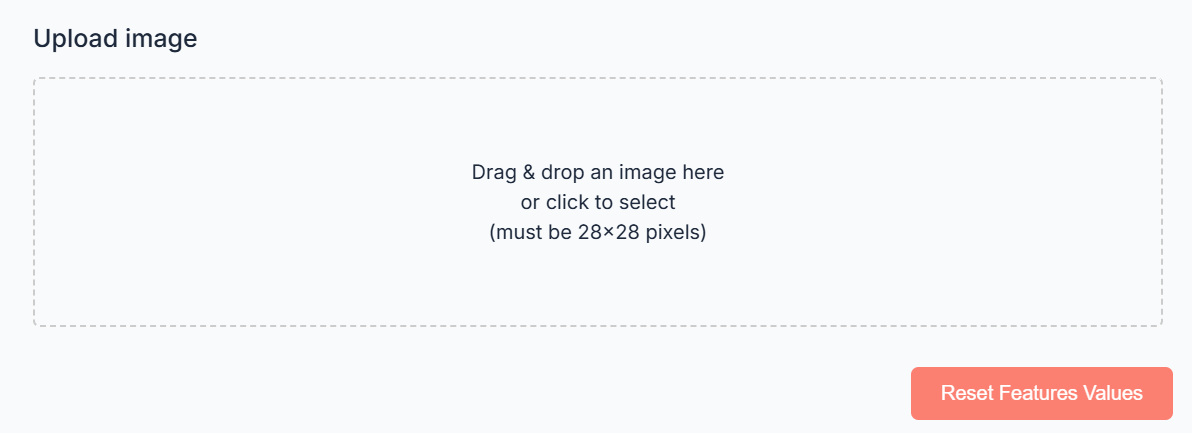
\includegraphics[width=\textwidth]{images/webapp image 1.png}
        \caption{When an image dataset was loaded the UI would change, allowing the user to upload an image instead of inputting the features.}
    \end{subfigure}
    \hfill
    \begin{subfigure}[c]{0.45\textwidth}
        \centering
        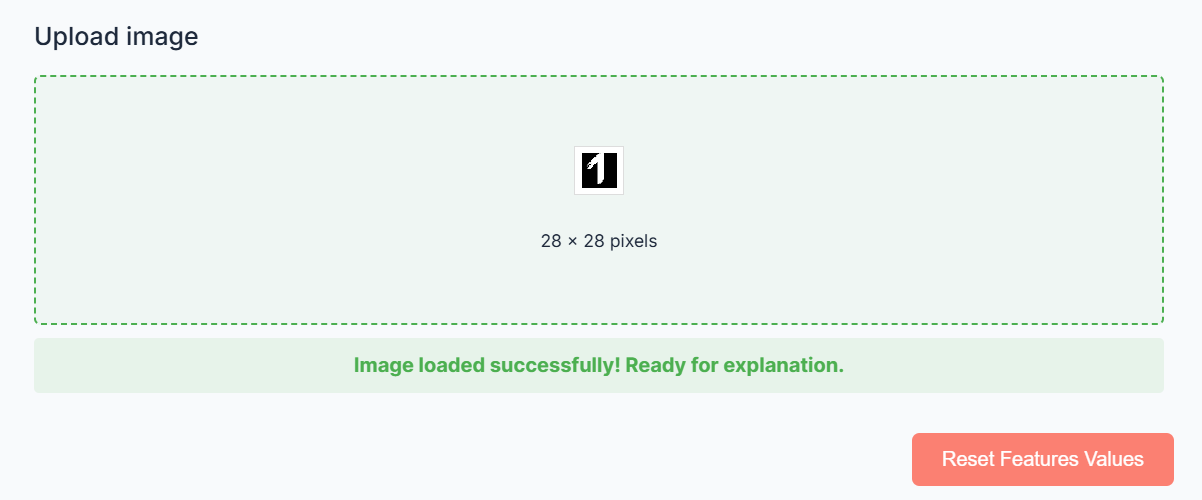
\includegraphics[width=\textwidth]{images/webapp image 3.png}
        \caption{Image uploaded correctly.}
    \end{subfigure}
    
    \vskip\baselineskip
    \begin{subfigure}[c]{\textwidth}
        \centering
        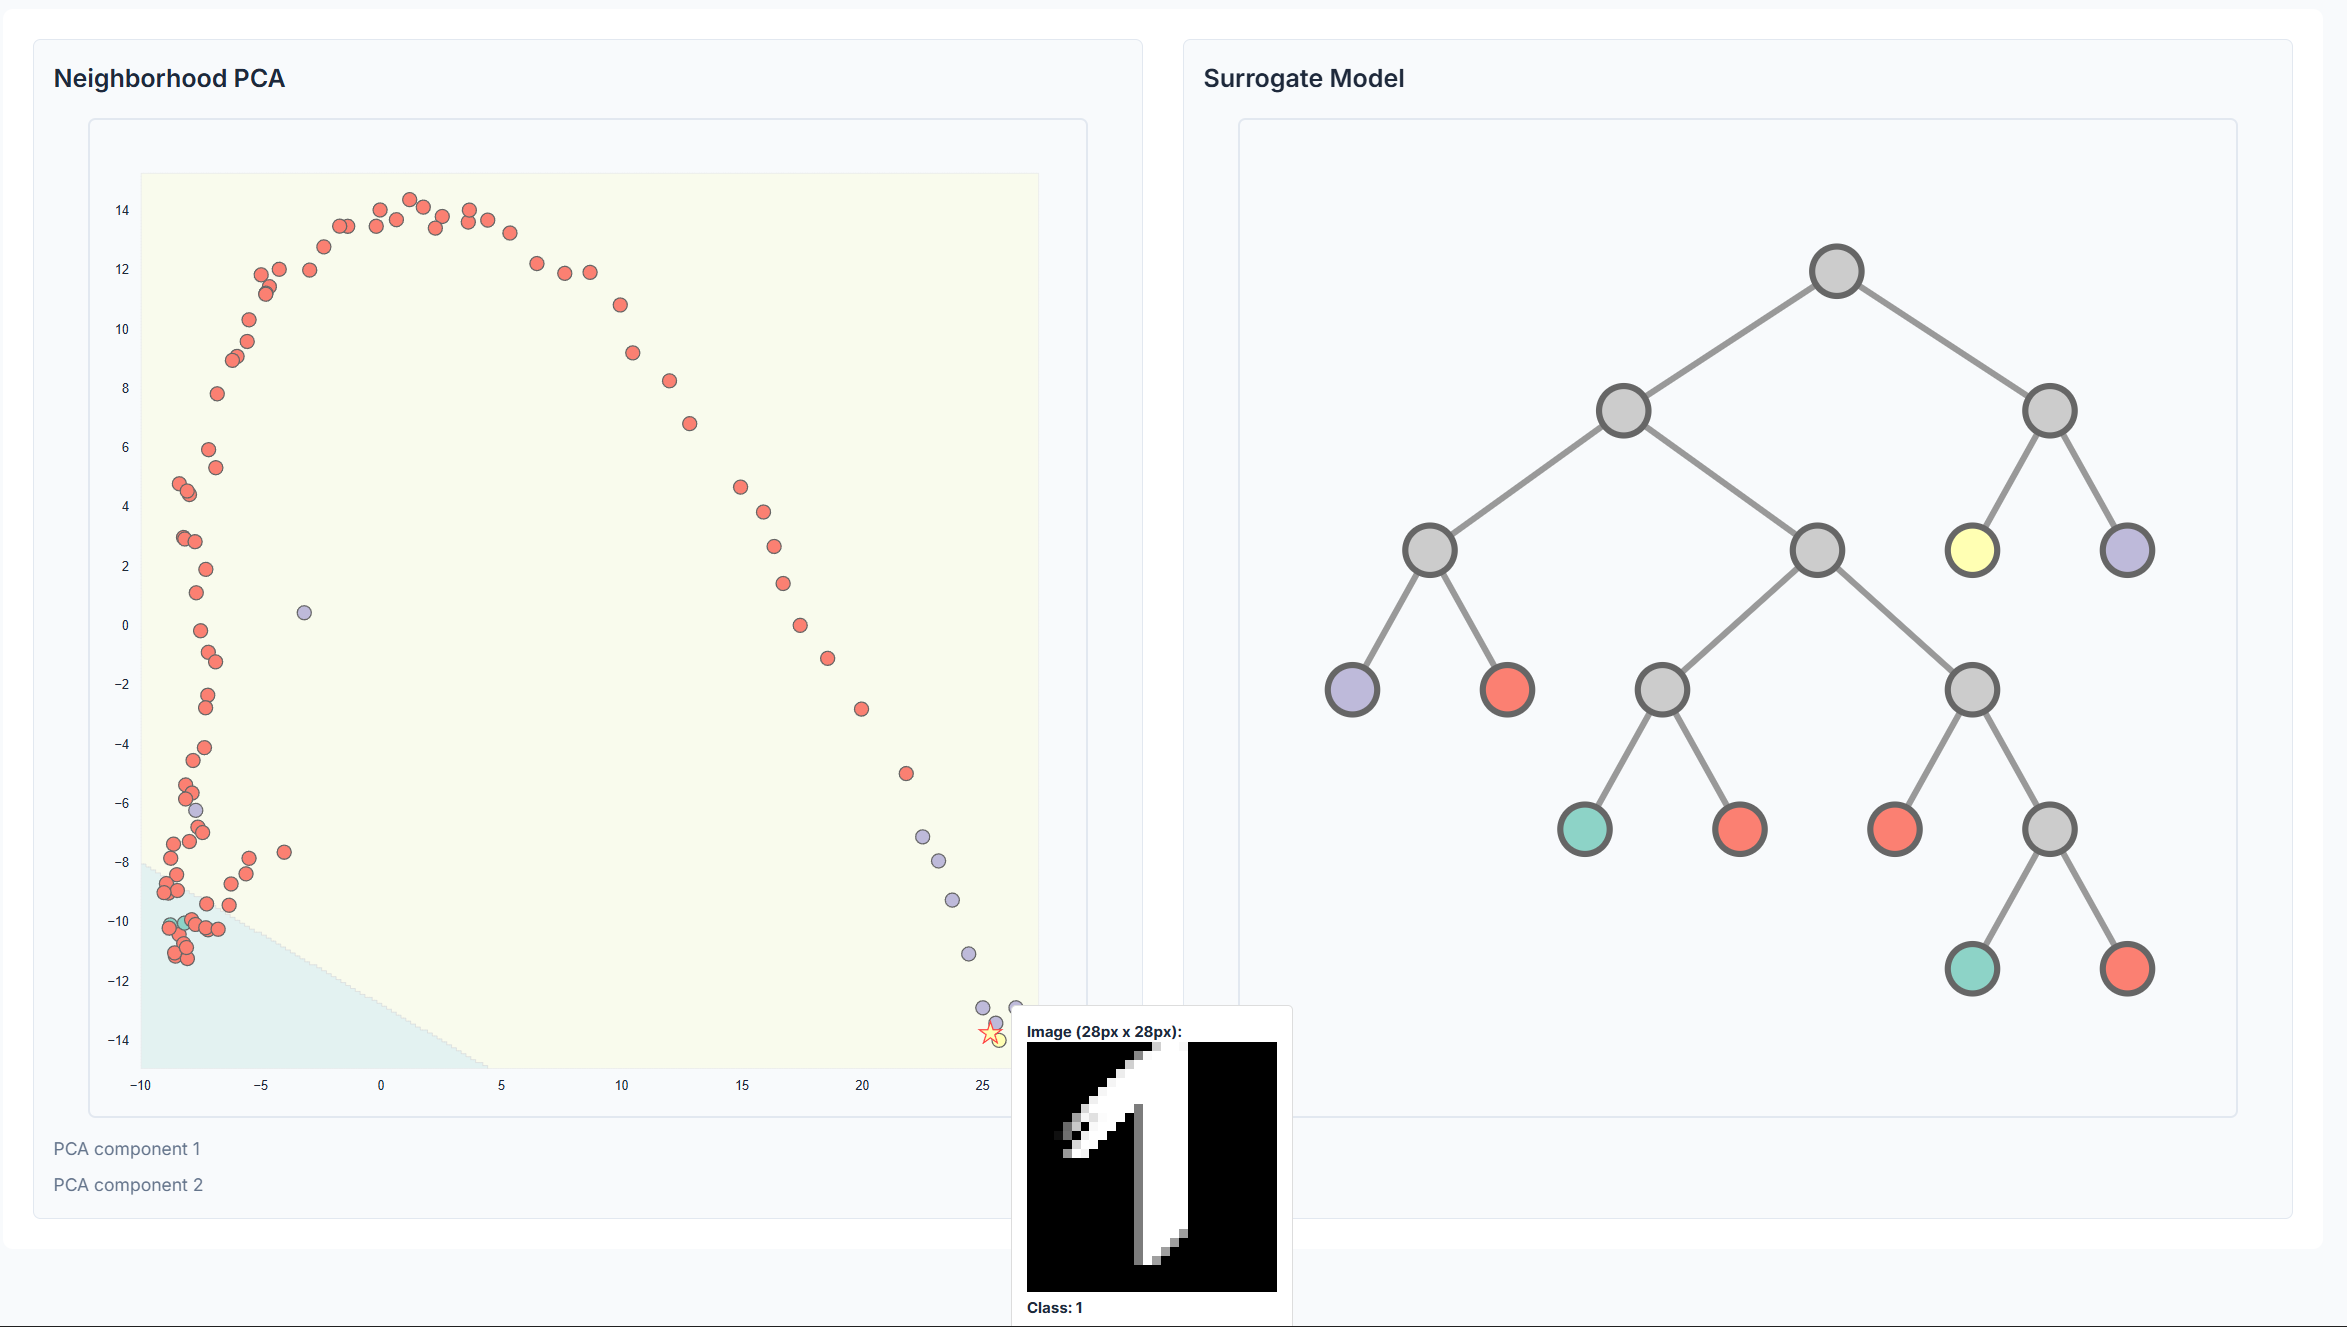
\includegraphics[width=\textwidth]{images/webapp image 4.png}
        \caption{The hover interaction on the points of the spatial neighborhood analysis plot would show the decoded images.}
    \end{subfigure}
    
    \caption{Experimental image-based interface prototype showing adaptive UI for image upload and pixel-level visualization in spatial neighborhood analysis plot interactions.}
    \label{fig:webappImgages}
\end{figure}
